% Created by tikzDevice version 0.12.6 on 2026-03-25 10:56:42
% !TEX encoding = UTF-8 Unicode
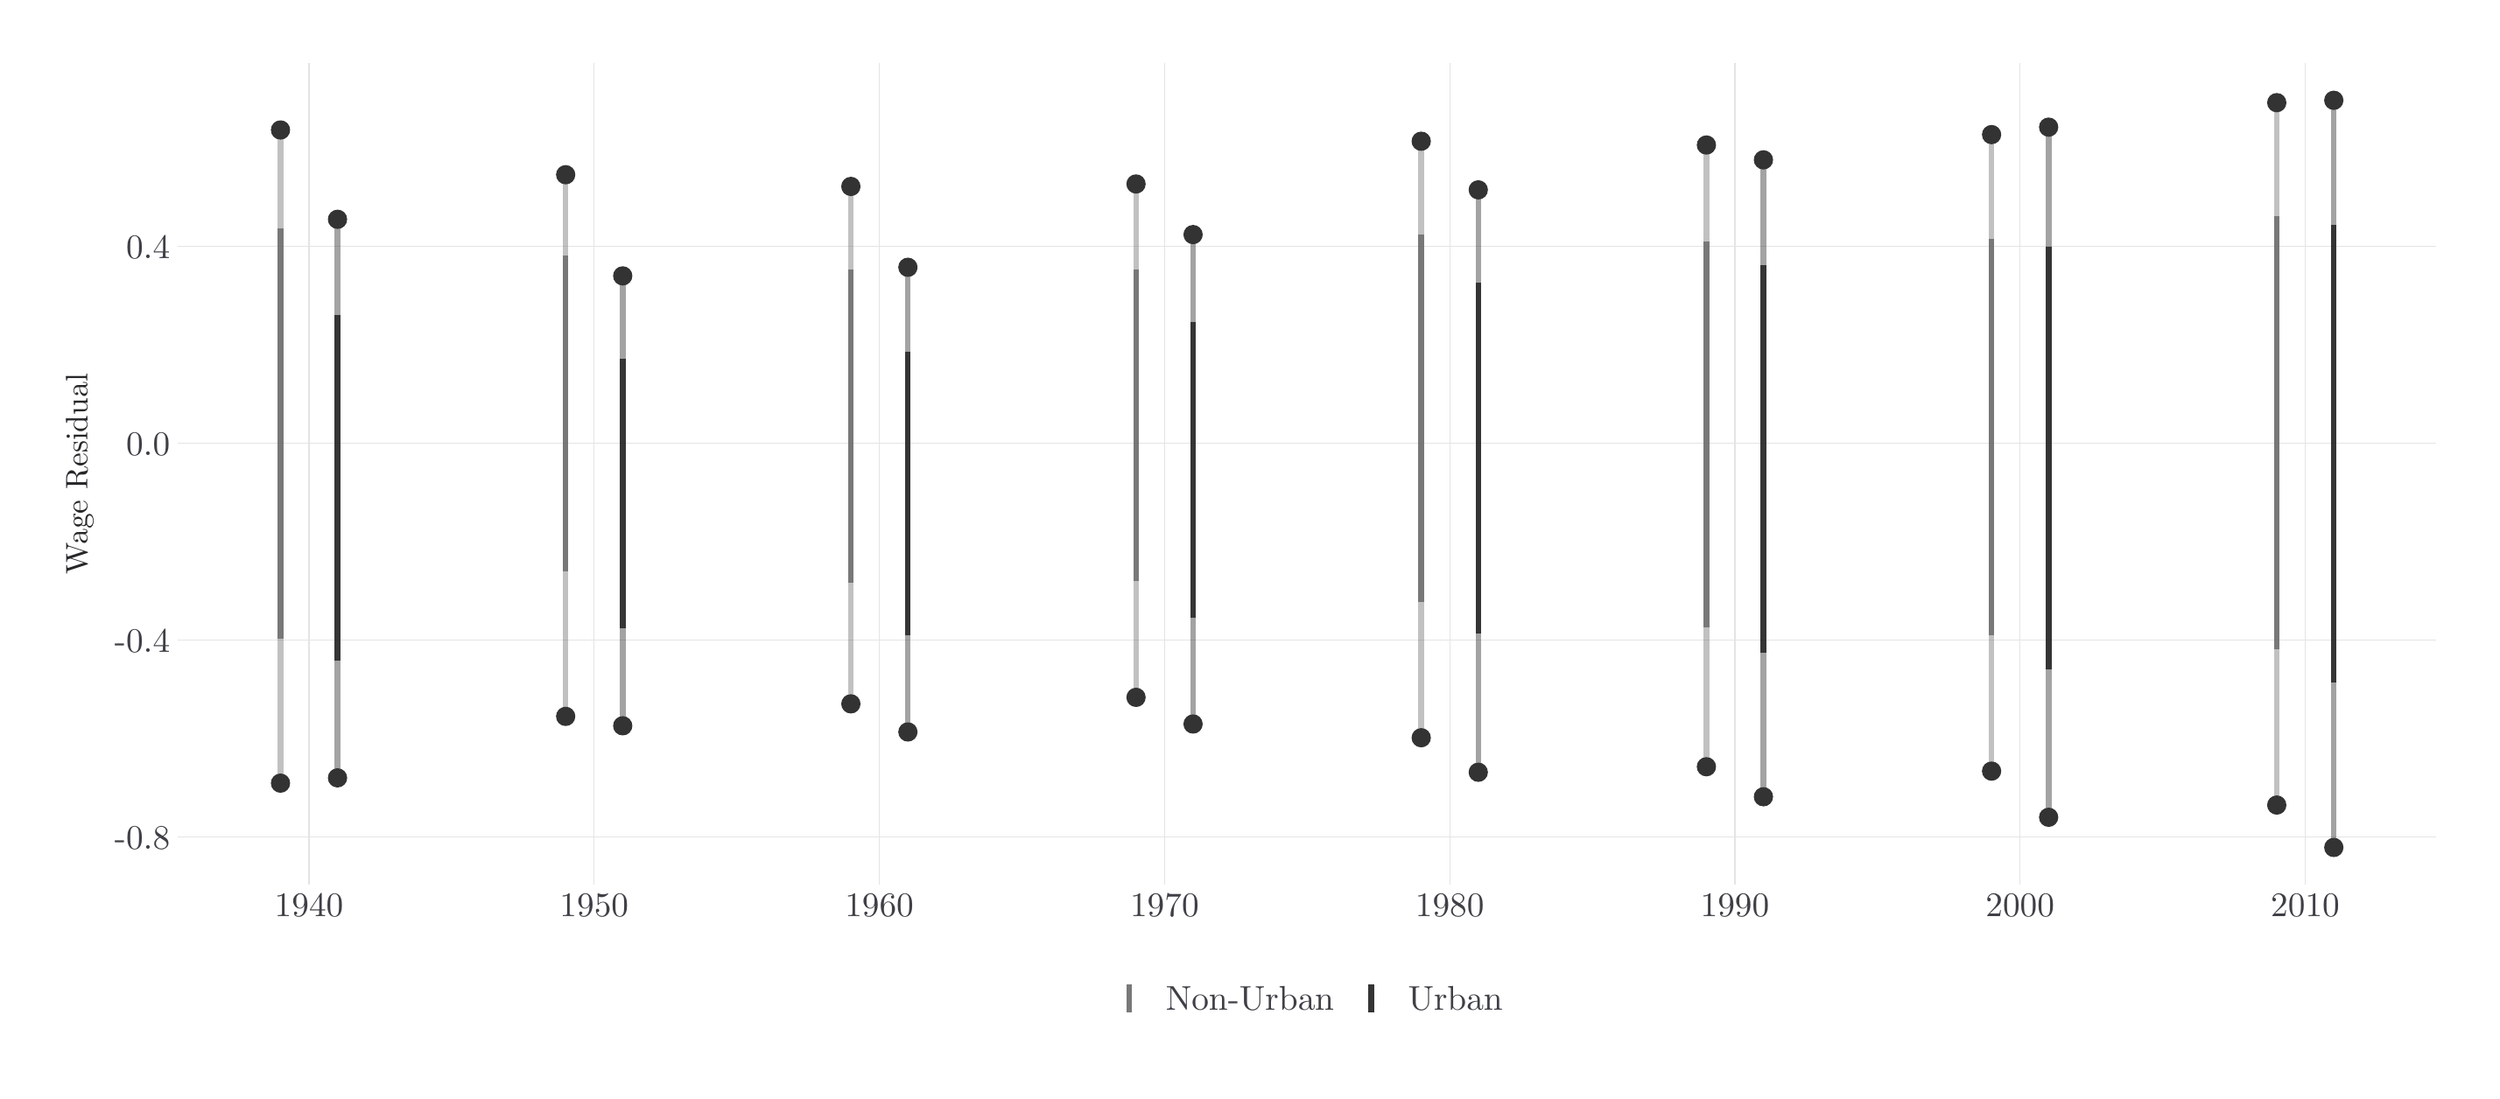
\begin{tikzpicture}[x=1pt,y=1pt]
\definecolor{fillColor}{RGB}{255,255,255}
\path[use as bounding box,fill=fillColor] (0,0) rectangle (1011.78,433.62);
\begin{scope}
\path[clip] (  0.00,  0.00) rectangle (1011.78,433.62);
\definecolor{drawColor}{RGB}{255,255,255}

\path[draw=drawColor,line width= 0.8pt,line join=round,line cap=round,fill=fillColor] (  0.00,  0.00) rectangle (1011.78,433.62);
\end{scope}
\begin{scope}
\path[clip] ( 63.41, 78.21) rectangle (995.78,417.62);
\definecolor{drawColor}{RGB}{255,255,255}
\definecolor{fillColor}{RGB}{255,255,255}

\path[draw=drawColor,line width= 0.8pt,line join=round,line cap=round,fill=fillColor] ( 63.41, 78.21) rectangle (995.78,417.62);
\definecolor{drawColor}{RGB}{228,228,231}

\path[draw=drawColor,line width= 0.4pt,line join=round] ( 63.41, 97.94) --
	(995.78, 97.94);

\path[draw=drawColor,line width= 0.4pt,line join=round] ( 63.41,179.26) --
	(995.78,179.26);

\path[draw=drawColor,line width= 0.4pt,line join=round] ( 63.41,260.58) --
	(995.78,260.58);

\path[draw=drawColor,line width= 0.4pt,line join=round] ( 63.41,341.89) --
	(995.78,341.89);

\path[draw=drawColor,line width= 0.4pt,line join=round] (117.56, 78.21) --
	(117.56,417.62);

\path[draw=drawColor,line width= 0.4pt,line join=round] (235.28, 78.21) --
	(235.28,417.62);

\path[draw=drawColor,line width= 0.4pt,line join=round] (353.01, 78.21) --
	(353.01,417.62);

\path[draw=drawColor,line width= 0.4pt,line join=round] (470.73, 78.21) --
	(470.73,417.62);

\path[draw=drawColor,line width= 0.4pt,line join=round] (588.46, 78.21) --
	(588.46,417.62);

\path[draw=drawColor,line width= 0.4pt,line join=round] (706.18, 78.21) --
	(706.18,417.62);

\path[draw=drawColor,line width= 0.4pt,line join=round] (823.90, 78.21) --
	(823.90,417.62);

\path[draw=drawColor,line width= 0.4pt,line join=round] (941.63, 78.21) --
	(941.63,417.62);
\definecolor{drawColor}{RGB}{26,26,26}

\path[draw=drawColor,draw opacity=0.40,line width= 2.3pt,line join=round] (129.33,122.38) -- (129.33,353.05);
\definecolor{drawColor}{RGB}{102,102,102}

\path[draw=drawColor,draw opacity=0.40,line width= 2.3pt,line join=round] (105.79,120.20) -- (105.79,389.94);
\definecolor{drawColor}{RGB}{26,26,26}

\path[draw=drawColor,draw opacity=0.40,line width= 2.3pt,line join=round] (247.06,143.88) -- (247.06,329.68);
\definecolor{drawColor}{RGB}{102,102,102}

\path[draw=drawColor,draw opacity=0.40,line width= 2.3pt,line join=round] (223.51,147.77) -- (223.51,371.46);
\definecolor{drawColor}{RGB}{26,26,26}

\path[draw=drawColor,draw opacity=0.40,line width= 2.3pt,line join=round] (364.78,141.34) -- (364.78,333.23);
\definecolor{drawColor}{RGB}{102,102,102}

\path[draw=drawColor,draw opacity=0.40,line width= 2.3pt,line join=round] (341.24,152.95) -- (341.24,366.62);
\definecolor{drawColor}{RGB}{26,26,26}

\path[draw=drawColor,draw opacity=0.40,line width= 2.3pt,line join=round] (482.50,144.62) -- (482.50,346.74);
\definecolor{drawColor}{RGB}{102,102,102}

\path[draw=drawColor,draw opacity=0.40,line width= 2.3pt,line join=round] (458.96,155.63) -- (458.96,367.64);
\definecolor{drawColor}{RGB}{26,26,26}

\path[draw=drawColor,draw opacity=0.40,line width= 2.3pt,line join=round] (600.23,124.70) -- (600.23,365.21);
\definecolor{drawColor}{RGB}{102,102,102}

\path[draw=drawColor,draw opacity=0.40,line width= 2.3pt,line join=round] (576.68,138.95) -- (576.68,385.29);
\definecolor{drawColor}{RGB}{26,26,26}

\path[draw=drawColor,draw opacity=0.40,line width= 2.3pt,line join=round] (717.95,114.58) -- (717.95,377.60);
\definecolor{drawColor}{RGB}{102,102,102}

\path[draw=drawColor,draw opacity=0.40,line width= 2.3pt,line join=round] (694.41,126.98) -- (694.41,383.73);
\definecolor{drawColor}{RGB}{26,26,26}

\path[draw=drawColor,draw opacity=0.40,line width= 2.3pt,line join=round] (835.68,106.10) -- (835.68,391.11);
\definecolor{drawColor}{RGB}{102,102,102}

\path[draw=drawColor,draw opacity=0.40,line width= 2.3pt,line join=round] (812.13,125.17) -- (812.13,388.03);
\definecolor{drawColor}{RGB}{26,26,26}

\path[draw=drawColor,draw opacity=0.40,line width= 2.3pt,line join=round] (953.40, 93.64) -- (953.40,402.19);
\definecolor{drawColor}{RGB}{102,102,102}

\path[draw=drawColor,draw opacity=0.40,line width= 2.3pt,line join=round] (929.85,111.16) -- (929.85,401.22);
\definecolor{drawColor}{RGB}{26,26,26}

\path[draw=drawColor,draw opacity=0.80,line width= 2.3pt,line join=round] (129.33,170.63) -- (129.33,313.47);
\definecolor{drawColor}{RGB}{102,102,102}

\path[draw=drawColor,draw opacity=0.80,line width= 2.3pt,line join=round] (105.79,179.66) -- (105.79,349.17);
\definecolor{drawColor}{RGB}{26,26,26}

\path[draw=drawColor,draw opacity=0.80,line width= 2.3pt,line join=round] (247.06,184.00) -- (247.06,295.29);
\definecolor{drawColor}{RGB}{102,102,102}

\path[draw=drawColor,draw opacity=0.80,line width= 2.3pt,line join=round] (223.51,207.60) -- (223.51,337.93);
\definecolor{drawColor}{RGB}{26,26,26}

\path[draw=drawColor,draw opacity=0.80,line width= 2.3pt,line join=round] (364.78,181.16) -- (364.78,298.18);
\definecolor{drawColor}{RGB}{102,102,102}

\path[draw=drawColor,draw opacity=0.80,line width= 2.3pt,line join=round] (341.24,202.95) -- (341.24,332.35);
\definecolor{drawColor}{RGB}{26,26,26}

\path[draw=drawColor,draw opacity=0.80,line width= 2.3pt,line join=round] (482.50,188.33) -- (482.50,310.47);
\definecolor{drawColor}{RGB}{102,102,102}

\path[draw=drawColor,draw opacity=0.80,line width= 2.3pt,line join=round] (458.96,203.54) -- (458.96,332.18);
\definecolor{drawColor}{RGB}{26,26,26}

\path[draw=drawColor,draw opacity=0.80,line width= 2.3pt,line join=round] (600.23,182.03) -- (600.23,326.92);
\definecolor{drawColor}{RGB}{102,102,102}

\path[draw=drawColor,draw opacity=0.80,line width= 2.3pt,line join=round] (576.68,195.05) -- (576.68,346.64);
\definecolor{drawColor}{RGB}{26,26,26}

\path[draw=drawColor,draw opacity=0.80,line width= 2.3pt,line join=round] (717.95,173.89) -- (717.95,334.07);
\definecolor{drawColor}{RGB}{102,102,102}

\path[draw=drawColor,draw opacity=0.80,line width= 2.3pt,line join=round] (694.41,184.54) -- (694.41,343.88);
\definecolor{drawColor}{RGB}{26,26,26}

\path[draw=drawColor,draw opacity=0.80,line width= 2.3pt,line join=round] (835.68,167.25) -- (835.68,341.62);
\definecolor{drawColor}{RGB}{102,102,102}

\path[draw=drawColor,draw opacity=0.80,line width= 2.3pt,line join=round] (812.13,181.24) -- (812.13,344.80);
\definecolor{drawColor}{RGB}{26,26,26}

\path[draw=drawColor,draw opacity=0.80,line width= 2.3pt,line join=round] (953.40,161.70) -- (953.40,350.81);
\definecolor{drawColor}{RGB}{102,102,102}

\path[draw=drawColor,draw opacity=0.80,line width= 2.3pt,line join=round] (929.85,175.53) -- (929.85,354.34);
\definecolor{drawColor}{gray}{0.20}
\definecolor{fillColor}{gray}{0.20}

\path[draw=drawColor,line width= 0.5pt,line join=round,line cap=round,fill=fillColor] (129.33,353.05) circle (  3.73);

\path[draw=drawColor,line width= 0.5pt,line join=round,line cap=round,fill=fillColor] (105.79,389.94) circle (  3.73);

\path[draw=drawColor,line width= 0.5pt,line join=round,line cap=round,fill=fillColor] (247.06,329.68) circle (  3.73);

\path[draw=drawColor,line width= 0.5pt,line join=round,line cap=round,fill=fillColor] (223.51,371.46) circle (  3.73);

\path[draw=drawColor,line width= 0.5pt,line join=round,line cap=round,fill=fillColor] (364.78,333.23) circle (  3.73);

\path[draw=drawColor,line width= 0.5pt,line join=round,line cap=round,fill=fillColor] (341.24,366.62) circle (  3.73);

\path[draw=drawColor,line width= 0.5pt,line join=round,line cap=round,fill=fillColor] (482.50,346.74) circle (  3.73);

\path[draw=drawColor,line width= 0.5pt,line join=round,line cap=round,fill=fillColor] (458.96,367.64) circle (  3.73);

\path[draw=drawColor,line width= 0.5pt,line join=round,line cap=round,fill=fillColor] (600.23,365.21) circle (  3.73);

\path[draw=drawColor,line width= 0.5pt,line join=round,line cap=round,fill=fillColor] (576.68,385.29) circle (  3.73);

\path[draw=drawColor,line width= 0.5pt,line join=round,line cap=round,fill=fillColor] (717.95,377.60) circle (  3.73);

\path[draw=drawColor,line width= 0.5pt,line join=round,line cap=round,fill=fillColor] (694.41,383.73) circle (  3.73);

\path[draw=drawColor,line width= 0.5pt,line join=round,line cap=round,fill=fillColor] (835.68,391.11) circle (  3.73);

\path[draw=drawColor,line width= 0.5pt,line join=round,line cap=round,fill=fillColor] (812.13,388.03) circle (  3.73);

\path[draw=drawColor,line width= 0.5pt,line join=round,line cap=round,fill=fillColor] (953.40,402.19) circle (  3.73);

\path[draw=drawColor,line width= 0.5pt,line join=round,line cap=round,fill=fillColor] (929.85,401.22) circle (  3.73);

\path[draw=drawColor,line width= 0.5pt,line join=round,line cap=round,fill=fillColor] (129.33,122.38) circle (  3.73);

\path[draw=drawColor,line width= 0.5pt,line join=round,line cap=round,fill=fillColor] (105.79,120.20) circle (  3.73);

\path[draw=drawColor,line width= 0.5pt,line join=round,line cap=round,fill=fillColor] (247.06,143.88) circle (  3.73);

\path[draw=drawColor,line width= 0.5pt,line join=round,line cap=round,fill=fillColor] (223.51,147.77) circle (  3.73);

\path[draw=drawColor,line width= 0.5pt,line join=round,line cap=round,fill=fillColor] (364.78,141.34) circle (  3.73);

\path[draw=drawColor,line width= 0.5pt,line join=round,line cap=round,fill=fillColor] (341.24,152.95) circle (  3.73);

\path[draw=drawColor,line width= 0.5pt,line join=round,line cap=round,fill=fillColor] (482.50,144.62) circle (  3.73);

\path[draw=drawColor,line width= 0.5pt,line join=round,line cap=round,fill=fillColor] (458.96,155.63) circle (  3.73);

\path[draw=drawColor,line width= 0.5pt,line join=round,line cap=round,fill=fillColor] (600.23,124.70) circle (  3.73);

\path[draw=drawColor,line width= 0.5pt,line join=round,line cap=round,fill=fillColor] (576.68,138.95) circle (  3.73);

\path[draw=drawColor,line width= 0.5pt,line join=round,line cap=round,fill=fillColor] (717.95,114.58) circle (  3.73);

\path[draw=drawColor,line width= 0.5pt,line join=round,line cap=round,fill=fillColor] (694.41,126.98) circle (  3.73);

\path[draw=drawColor,line width= 0.5pt,line join=round,line cap=round,fill=fillColor] (835.68,106.10) circle (  3.73);

\path[draw=drawColor,line width= 0.5pt,line join=round,line cap=round,fill=fillColor] (812.13,125.17) circle (  3.73);

\path[draw=drawColor,line width= 0.5pt,line join=round,line cap=round,fill=fillColor] (953.40, 93.64) circle (  3.73);

\path[draw=drawColor,line width= 0.5pt,line join=round,line cap=round,fill=fillColor] (929.85,111.16) circle (  3.73);
\end{scope}
\begin{scope}
\path[clip] (  0.00,  0.00) rectangle (1011.78,433.62);
\definecolor{drawColor}{RGB}{63,63,70}

\node[text=drawColor,anchor=base east,inner sep=0pt, outer sep=0pt, scale=  1.42] at ( 60.21, 93.05) {-0.8};

\node[text=drawColor,anchor=base east,inner sep=0pt, outer sep=0pt, scale=  1.42] at ( 60.21,174.36) {-0.4};

\node[text=drawColor,anchor=base east,inner sep=0pt, outer sep=0pt, scale=  1.42] at ( 60.21,255.68) {0.0};

\node[text=drawColor,anchor=base east,inner sep=0pt, outer sep=0pt, scale=  1.42] at ( 60.21,336.99) {0.4};
\end{scope}
\begin{scope}
\path[clip] (  0.00,  0.00) rectangle (1011.78,433.62);
\definecolor{drawColor}{RGB}{63,63,70}

\node[text=drawColor,anchor=base,inner sep=0pt, outer sep=0pt, scale=  1.42] at (117.56, 65.22) {1940};

\node[text=drawColor,anchor=base,inner sep=0pt, outer sep=0pt, scale=  1.42] at (235.28, 65.22) {1950};

\node[text=drawColor,anchor=base,inner sep=0pt, outer sep=0pt, scale=  1.42] at (353.01, 65.22) {1960};

\node[text=drawColor,anchor=base,inner sep=0pt, outer sep=0pt, scale=  1.42] at (470.73, 65.22) {1970};

\node[text=drawColor,anchor=base,inner sep=0pt, outer sep=0pt, scale=  1.42] at (588.46, 65.22) {1980};

\node[text=drawColor,anchor=base,inner sep=0pt, outer sep=0pt, scale=  1.42] at (706.18, 65.22) {1990};

\node[text=drawColor,anchor=base,inner sep=0pt, outer sep=0pt, scale=  1.42] at (823.90, 65.22) {2000};

\node[text=drawColor,anchor=base,inner sep=0pt, outer sep=0pt, scale=  1.42] at (941.63, 65.22) {2010};
\end{scope}
\begin{scope}
\path[clip] (  0.00,  0.00) rectangle (1011.78,433.62);
\definecolor{drawColor}{RGB}{39,39,42}

\node[text=drawColor,rotate= 90.00,anchor=base,inner sep=0pt, outer sep=0pt, scale=  1.28] at ( 26.06,247.92) {Wage Residual};
\end{scope}
\begin{scope}
\path[clip] (  0.00,  0.00) rectangle (1011.78,433.62);
\definecolor{drawColor}{RGB}{255,255,255}
\definecolor{fillColor}{RGB}{255,255,255}

\path[draw=drawColor,line width= 0.8pt,line join=round,line cap=round,fill=fillColor] (440.80, 16.00) rectangle (618.39, 46.45);
\end{scope}
\begin{scope}
\path[clip] (  0.00,  0.00) rectangle (1011.78,433.62);
\definecolor{drawColor}{RGB}{255,255,255}
\definecolor{fillColor}{RGB}{255,255,255}

\path[draw=drawColor,line width= 0.8pt,line join=round,line cap=round,fill=fillColor] (448.80, 24.00) rectangle (463.26, 38.45);
\definecolor{drawColor}{RGB}{102,102,102}

\path[draw=drawColor,draw opacity=0.40,line width= 2.3pt,line join=round] (456.03, 25.45) -- (456.03, 37.01);
\definecolor{drawColor}{RGB}{102,102,102}

\path[draw=drawColor,draw opacity=0.80,line width= 2.3pt,line join=round] (456.03, 25.45) -- (456.03, 37.01);
\end{scope}
\begin{scope}
\path[clip] (  0.00,  0.00) rectangle (1011.78,433.62);
\definecolor{drawColor}{RGB}{255,255,255}
\definecolor{fillColor}{RGB}{255,255,255}

\path[draw=drawColor,line width= 0.8pt,line join=round,line cap=round,fill=fillColor] (548.80, 24.00) rectangle (563.25, 38.45);
\definecolor{drawColor}{RGB}{26,26,26}

\path[draw=drawColor,draw opacity=0.40,line width= 2.3pt,line join=round] (556.02, 25.45) -- (556.02, 37.01);
\definecolor{drawColor}{RGB}{26,26,26}

\path[draw=drawColor,draw opacity=0.80,line width= 2.3pt,line join=round] (556.02, 25.45) -- (556.02, 37.01);
\end{scope}
\begin{scope}
\path[clip] (  0.00,  0.00) rectangle (1011.78,433.62);
\definecolor{drawColor}{RGB}{63,63,70}

\node[text=drawColor,anchor=base west,inner sep=0pt, outer sep=0pt, scale=  1.42] at (471.26, 26.33) {Non-Urban};
\end{scope}
\begin{scope}
\path[clip] (  0.00,  0.00) rectangle (1011.78,433.62);
\definecolor{drawColor}{RGB}{63,63,70}

\node[text=drawColor,anchor=base west,inner sep=0pt, outer sep=0pt, scale=  1.42] at (571.25, 26.33) {Urban};
\end{scope}
\end{tikzpicture}
